\documentclass[12pt]{article}
\usepackage{amsmath}
\usepackage{graphicx}
\usepackage{wrapfig}
\usepackage{booktabs}
\usepackage[letterpaper, margin=1in]{geometry}
\usepackage{fancyhdr}
\pagestyle{fancy}
\fancyhead[R]{Inductors and Capacitors}
\fancyfoot[C]{\thepage}
\renewcommand{\headrulewidth}{1pt}
\renewcommand{\footrulewidth}{1pt}
\usepackage [autostyle, english = american]{csquotes}
\MakeOuterQuote{"}
\renewcommand{\baselinestretch}{1.0}
\newcommand{\twoobjects}[2]{%
  \leavevmode\vbox{\hbox{#1}\nointerlineskip\hbox{#2}}%
}
\begin{document}
    \section*{The Inductor}
    \[
        v(t) = L \frac{di}{dt}
    \]
    \par The voltage across an inductor is given by the equation above and from
    this the expression for the current across an inductor can also be derived
    by separating variables and integrating both sides.
    \[
        i(t) = \frac{1}{L} \int v(t)\ dt = \frac{1}{L} \int_{-\infty}^t v(\tau)\
        d\tau
    \]
    \par One thing to note is the behavior of on inductor in the presence of a
    dc power supply. If the current across the inductor is constant, the voltage
    across it will be zero. This implicates that an inductor in the presence of
    a constant dc current source will behave the same as a short circuit in its
    place. This fact also makes it clear that the current across an inductor
    cannot change instantaneously since the derivative at that point would not
    exist. The \textbf{current} in an inductor \textbf{must be continuous.}
    \par For the equation calculating current, it is not ideal to integrate for
    an infinite amount of time since the inductor will reach a steady state at
    some point as well as the fact that the interval of time that is of interest
    in not all of time. To rewrite this, the integral can be written as going
    from the initial time to some time $t$ and an initial condition can be
    specified which is added on to the end of the expression.
    \[
        i(t) = \frac{1}{L} \int_{t_0}^t v(\tau)\ d\tau + i(t_0)
    \]
    \par Most of the time this requires the functions to be defined as a
    piecewise functions, and it is imperative to make explicit that for an
    inductor, current cannot be discontinuous however, voltage can.
    \subsection*{Power and Energy}
    The power stored in an inductor is calculated using $p=iv$ and since
    $v = L \frac{di}{dt}$, the power is given as,
    \[
        p = Li \frac{di}{dt}
    .\]
    The energy in an inductor is given by,
    \[
        w = \frac{1}{2} Li^2
    .\]
    \newpage
    \section*{The Capacitor}
    \[
        i(t) = C \frac{dv}{dt}
    \]
    \par For a capacitor, somewhat the opposite is given by the equations, the
    current is the capacitance multiplied with the derivative of the voltage
    across the capacitor. Examining this the same as with the inductor, here it
    can be seen that since the voltage is being differentiated, the function for
    the voltage, \textbf{cannot be discontinuous.}
    \par For the current, the same is
    done, separation of variables and then integration, and the following
    expression is received,
    \[
        v(t) = \frac{1}{C} \int_{t_0}^t i(\tau)\ d\tau + v(t_0)
    .\]
    \par The same can be said for this conversion and the same rules apply. In
    this case, the current can be given as a discontinuous function however, the
    voltage cannot.
    \subsection*{Power and Energy}
    Power is defined much the same way, since $p=vi$,
    \[
        p = Cv \frac{dv}{dt}
    \]
    Energy is also much the same exert this time,
    \[
        w = \frac{1}{2} Cv^2
    \]
    \section*{Appendix G Integrals}
    \;
    \[
        \int xe^{ax}\ dx = \frac{e^{ax}}{a^2} (ax-1)
    \]
    \\
    \[
        \int x^2 e^{ax}\ dx = \frac{e^{ax}}{a^3} (a^2 x^2 - 2ax + 2)
    \]
    \\
    \[
        \int x\sin (ax)\ dx = \frac{1}{a^2} \sin (ax) - \frac{x}{a} \cos (ax)
    \]
    \\
    \[
        \int x\cos (ax)\ dx = \frac{1}{a^2} \cos (ax) - \frac{x}{a} \sin (ax)
    \]
    \newpage
    \section*{Mutual Inductance}
    \begin{figure}[h]
        \centering
        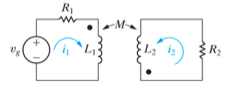
\includegraphics[width=0.5\textwidth]{Coupled Inductors.png}
    \end{figure}
    \par The inductors in this circuit are magnetically coupled due to them
    being in close proximity with one another. This causes the original mesh
    equations to be altered to accommodate the voltage induced by the opposing
    inductor. The original mesh equations written for the independent circuits
    would be, $-v_g + i_1R_1 + L_1 \frac{di_1}{dt} = 0$ for the one on the left,
    and for the right, $i_2R_2 + L_2 \frac{di_2}{dt} = 0$.
    \par Now since these inductors are close to each other and each induce
    voltage on the other, another term must be added to each of their equations.
    For the circuit on the left, since the current $i_2$ travels into the
    negative polar side of the inductor, indicated by the dot, the term for the
    voltage induced will be negative. This gives the new equation,
    \[
        -v_g + i_1R_1 + L_1 \frac{di_1}{dt} - M \frac{di_2}{dt} = 0
    .\]
    \par The same must be done for the second equation and in this case, since
    $i_1$ travels into the positive end of $L_1$, the positive emf is generated
    at the positive end of the other inductor. Since the current $i_2$ is
    entering the negative end of that inductor, the term in the second equation
    will be negative.
    \[
        i_2R_2 + L_2 \frac{di_2}{dt} - M \frac{di_1}{dt} = 0
    \]
    \subsection*{Dot Placement}
    \begin{figure}[h]
        \centering
        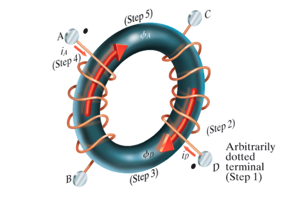
\includegraphics[width=0.35\textwidth]{Dot Selection.png}
    \end{figure}
    \par The placement of the dots for the positive and negative ends of the
    inductor is dependent on the direction of the flux that is traveling through
    the coil of the circuit. To determine which ends of the inductor are paired,
    use the right hand rule following the coils of the inductor with the curling
    of your fingers. The direction your thumb points is the direction the flux
    is traveling through the circuit. Do the same for the rest of the ends and
    which ever ones produce flux that travels in the same direction, are the
    ones that are coupled and that is where the dots should be placed.
    \subsection*{Derivation of Mutual Inductance}
    \[
        \varepsilon = \frac{d\lambda}{dt}
    \]
    \par The concept of mutual inductance stems as a result of Faraday's Law
    where, an emf is induced according to the rate of change of the magnetic
    flux within a coil. In simpler terms, if there is a change in the amount of
    flux generated within an electrically conductive material, there will be a
    voltage generated as a result.
    \par The term $\lambda$ represents flux linkage and is given by the
    equation, $\lambda = \phi N$. The magnitude of the flux is given by the
    equation $\phi = \mathcal{P} N i$, where $N$ is the number of turns the coil
    makes and $\mathcal{P}$ is the permeance of the region the flux is
    intersecting. Plugging these expressions into Faraday's Law, the equation
    for the current within an inductor can be derived.
    \begin{align*}
        v & = \frac{d\lambda}{dt} = \frac{d(N\phi)}{dt}, \\
          & = N \frac{d\phi}{dt} = N \frac{d}{dt}(\mathcal{P}Ni), \\
          & = N^2 \mathcal{P} \frac{di}{dt} = L \frac{di}{dt}.
    \end{align*}
    \par It can be determined from here that the term for inductance, $L$, is
    given by $N^2\mathcal{P}$. Further, we can derive the term for mutual
    inductance, $M$, which is actually responsible for the coupling of the two
    coils.
    \begin{figure}[h]
        \centering
        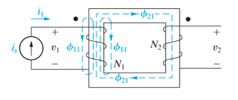
\includegraphics[width=0.4\textwidth]{Coupled Coils.png}
    \end{figure}
    \par The total flux in the first coil can be written as the sum of the flux
    generated by the coil and the flux traveling through the medium,
    \[
        \phi_1 = \phi_{11} + \phi_{21}
    .\]
    \par Now, each of the flux terms can be written as their full expressions,
    \[
        \phi_1 = \mathcal{P}_1 N_1 i_1,
    \]
    \[
        \phi_{11} = \mathcal{P}_{11} N_1 i_1,
    \]
    \[
        \phi_{21} = \mathcal{P}_{21} N_1 i_1.
    \]
    \par Here, $\mathcal{P}_1$ is the permeance of space occupied by the flux
    $\phi_1$, $\mathcal{P}_{11}$ is the permeance of the space through which
    $\phi_{11}$ travels, and $\mathcal{P}_{21}$ is the permeance of $\phi_{21}$.
    Using this, the equation relating the permeances of each of the fluxes can
    be written as,
    \[
        \mathcal{P}_1 = \mathcal{P}_{11} + \mathcal{P}_{21}
    .\]
    \par With this, Faraday's Law can be employed and with the same methodology
    as with the derivation of self-inductance, the term for mutual inductance
    can be determined.
    \begin{align*}
        v_1 &= \frac{d\lambda_1}{dt} = \frac{d(N_1\phi_1)}{dt} = N_1
            \frac{d}{dt}(\phi_{11} + \phi_{21}) \\
            &= N_1^2(\mathcal{P}_{11} + \mathcal{P}_{21}) \frac{di_1}{dt} =
            N_1^2 \mathcal{P}_1 \frac{di_1}{dt} = L_1 \frac{di_1}{dt}. \\
    \end{align*}
    \par For $v_2$ the same can be written, as this one was the derivation of
    the term for the self-inductance of the first inductor, the second equation
    will give the term for the induced voltage.
    \begin{align*}
        v_2 &= \frac{d\lambda_2}{dt} = \frac{d(N_2\phi_{21})}{dt} = N_2
            \frac{d}{dt} (\mathcal{P}_{21}N_1i_1) \\
            &= N_2 N_1 \mathcal{P}_{21} \frac{di_1}{dt} = M_{21}
            \frac{di_1}{dt}. \\
    \end{align*}
    \par Now it can be seen that the term $M$ is given by the product of the
    number of coils in each of the inductors, as well as the permeance of the
    medium through which the flux is traveling for both inductors.
    \[
        M_{21} = N_2 N_1 \mathcal{P}_{21}.
    \]
    \par The subscript on $M$ signifies that this is the inductance as it
    relates to the voltage induced in coil 2 by the current in coil 1. For
    non-magnetic materials, the permeances of both are equal, which means that
    the subscript does not matter and the term can be written as just simply,
    $M$.
    \subsection*{In terms of Self-Inductance}
    \[
        L_1 = N_1^2 \mathcal{P}_1,
    \]
    \[
        L_2 = N_2^2 \mathcal{P}_2,
    \]
    \[
        L_1 L_2 = N_1^2 N_2^2 \mathcal{P}_1 \mathcal{P}_2.
    \]
    \par These are the self-inductances for each of the two coils as well as
    their product. Using previous knowledge, this product can be rewritten in
    terms of the two individual permeances.
    \[
        L_1 L_2 = N_1^2 N_2^2 (\mathcal{P}_{11} +
        \mathcal{P}_{21})(\mathcal{P}_{22} + \mathcal{P}_{12})
    .\]
    \par Since for linear systems $\mathcal{P}_{21} = \mathcal{P}_{12}$, this
    expression can be simplified and written as,
    \[
        L_1 L_2 = (N_1N_2\mathcal{P}_{12})^2
        \left( 1 + \frac{\mathcal{P}_{11}}{\mathcal{P}_{12}} \right)
        \left( 1 + \frac{\mathcal{P}_{22}}{\mathcal{P}_{12}} \right)
    \]
    \par Here it can be seen that the definition for $M$ is present. Along with
    that, the self-inductance terms can be found by rearranging the product
    terms and with the use of a coefficient, $k$, the equation can be written
    as,
    \[
        \frac{1}{k^2} =
        \left( 1 + \frac{\mathcal{P}_{11}}{\mathcal{P}_{12}} \right)
        \left( 1 + \frac{\mathcal{P}_{22}}{\mathcal{P}_{12}} \right)
    ,\]
    rearranging,
    \[
        M^2 = k^2 L_1L_2
    ,\]
    \[
        M = k \sqrt{L_1L_2}
    .\]
    \par The coefficient $k$ is known as the \textit{coefficient of coupling}
    and it is defined within the range,
    \[
        0 \le k \le 1
    .\]
    \subsection*{Energy Stored in Coupled Coils}
    \[
        w(t) = \frac{1}{2} L_1 i_1^2 + \frac{1}{2} L_2 i_2^2 \pm Mi_1i_2
    .\]
\end{document}
